% ==============================================================================
% Mixture of Scars (MoS) & SCache O(1) — Official Academic Manuscript
% Compatible with: arXiv (cs.LG / cs.CL), TMLR, and Double-Blind Workshops
% ==============================================================================
\documentclass[10pt,twocolumn]{article}

% Toggle `\anonymoustrue` for Double-Blind Peer Review (NeurIPS/ICML/ICLR/TMLR)
% Keep `\anonymousfalse` for arXiv / Camera-Ready / Zenodo Preprint
\newif\ifanonymous
\anonymousfalse

\usepackage[utf8]{inputenc}
\usepackage[T1]{fontenc}
\usepackage{lmodern}
\usepackage{microtype}
\usepackage[margin=0.75in,columnsep=0.28in]{geometry}
\usepackage{amsmath,amssymb,amsfonts,amsthm}
\usepackage{mathtools}
\usepackage{booktabs}
\usepackage{multirow}
\usepackage{graphicx}
\usepackage{xcolor}
\usepackage{algorithm}
\usepackage{algorithmic}
\usepackage[numbers,sort&compress]{natbib}
\usepackage[colorlinks=true,linkcolor=blue!60!black,citecolor=blue!60!black,urlcolor=blue!65!black]{hyperref}

\newtheorem{proposition}{Proposition}
\newtheorem{remark}{Remark}

\title{\textbf{Mixture of Scars (MoS) and SCache $\mathcal{O}(1)$:\\Breaking the Dual Memory Wall of Modern Transformers via Activation-Aware Low-Rank Scar Experts and Widrow-Hoff Associative Memory}}

\ifanonymous
\author{
  \textbf{Anonymous Author(s)}\\
  Paper under double-blind review
}
\else
\author{
  \textbf{Julio Cesar Reis Filho}\\
  Byte-OD Research \& System One Architecture Lab\\
  \texttt{DOI: \href{https://doi.org/10.5281/zenodo.24143839}{10.5281/zenodo.24143839}} \quad|\quad
  \texttt{\href{https://github.com/byte-od/mixture-of-scars}{github.com/byte-od/mixture-of-scars}}
}
\fi

\date{November 11, 2026}

\begin{document}
\maketitle

\begin{abstract}
Autoregressive Large Language Models (LLMs) face a compounding \emph{Dual Memory Wall}: (i) a static parameter wall $\mathcal{O}(N)$ requiring tens to hundreds of gigabytes of VRAM to store frontier weights, and (ii) a dynamic context wall $\mathcal{O}(T)$ where key-value (KV) caches expand linearly with sequence length $T$. Existing post-training interventions typically address only one bottleneck in isolation---either suffering severe logit degradation on out-of-distribution activation outliers under 4-bit weight quantization, or permanently discarding evicted context tokens in fixed-window caches. We introduce two complementary primitives that break both walls simultaneously without retraining from scratch: (1) \textbf{Mixture of Scars (MoS)}, which pairs symmetric \texttt{INT4} base projections with compact ($<64$~KB) Activation-Aware Singular Value Decomposition (\texttt{ASVD}) residual ``scar'' experts and sequential layer-group streaming; and (2) \textbf{SCache (\texttt{SCacheDynamicCache})}, a drop-in $\mathcal{O}(1)$ constant-space dynamic cache combining attention sinks, a rolling local FIFO window, and per-KV-head associative fast-weight slots updated via the orthogonal \emph{Widrow-Hoff Delta Rule} with ReLU manifold gating and monotonic cumulative RoPE phase tracking. To prevent benchmark facades, we introduce a 7-vector \emph{Adversarial Red-Team Falsification Suite} enforcing recursive PyTorch storage-pointer byte audits ($0.00$~KB discrepancy) and mid-flight causality ablations across real pretrained Transformers (\texttt{Qwen2.5-0.5B-Instruct}, \texttt{Qwen2.5-72B-Instruct}, and \texttt{Mistral-Large-123B}). Empirically, \texttt{MoS} reduces single-model MLP RAM by $68.6\%$, cuts 8-specialist multi-tenant VRAM by $92.6\%$ ($13.58\times$), lowers unseen-domain logit KL divergence by $2.45\times$--$4.22\times$ over pure \texttt{INT4}, and streams 72B/123B backbones with $0.04$~GiB post-layer residual VRAM. Simultaneously, \texttt{SCache} enforces $+0.00$ marginal bytes beyond window saturation ($-91.4\%$ KV RAM at $L=1{,}280$), eliminates additive Hebbian ghosting ($\cos=1.0000$ vs.\ $0.467$), and achieves $22.58\times$ higher exact target probability on evicted passcodes than \texttt{StreamingLLM} with zero fine-tuning.
\end{abstract}

\section{Introduction}
Modern Transformer inference~\citep{vaswani2017attention} is governed by two simultaneous hardware bottlenecks. First, static parameters scale as $\mathcal{O}(N)$: a 72B-parameter model occupies $\sim 145$~GB in FP16/BF16 and $\sim 40$~GB even in 4-bit precision, exceeding commodity 8--24~GB GPUs. Second, autoregressive decoding caches explicit key-value tensors across all $L_{\text{layers}}$ layers and $H_{\text{kv}}$ grouped-query heads, consuming $\mathcal{O}(T \cdot L_{\text{layers}} \cdot H_{\text{kv}} \cdot d_{\text{head}})$ dynamic memory that grows unboundedly with sequence length $T$.

Prior efficiency methods tackle either static weights or dynamic context separately, introducing distinct failure modes under adversarial stress:
\begin{itemize}
    \item \textbf{Outlier fragility in static 4-bit quantization:} Uniform post-training \texttt{INT4} quantization suffers large logit KL divergence when heavy-tailed activation channels~\citep{lin2024awq,dettmers2023qlora} encounter unseen code, symbolic equations, or strict schemas.
    \item \textbf{Amnesia vs.\ ghosting in bounded context:} Sliding-window caches with attention sinks (\texttt{StreamingLLM}~\citep{xiao2024efficient}) stabilize perplexity but suffer total amnesia once a token exits the local window. Conversely, compressing evicted tokens via additive Hebbian outer products~\citep{schmidhuber1992learning} causes severe superposition interference (``ghosting'') whenever state variables mutate over time~\citep{schlag2021linear,yang2024parallelizing}.
\end{itemize}

In this paper, we unify static and dynamic compression around a shared geometric observation: bulk representational energy is compressible into coarse substrates (\texttt{INT4} bases and local windows), whereas high-leverage semantic deviations concentrate in low-rank directional residuals (\emph{scars}). Crucially, we evaluate both primitives under a hostile 7-vector Red-Team protocol designed explicitly to falsify $\mathcal{O}(1)$ memory claims, causal readout activity, out-of-domain robustness, and contradictory state overwrites.

\begin{figure*}[t]
    \centering
    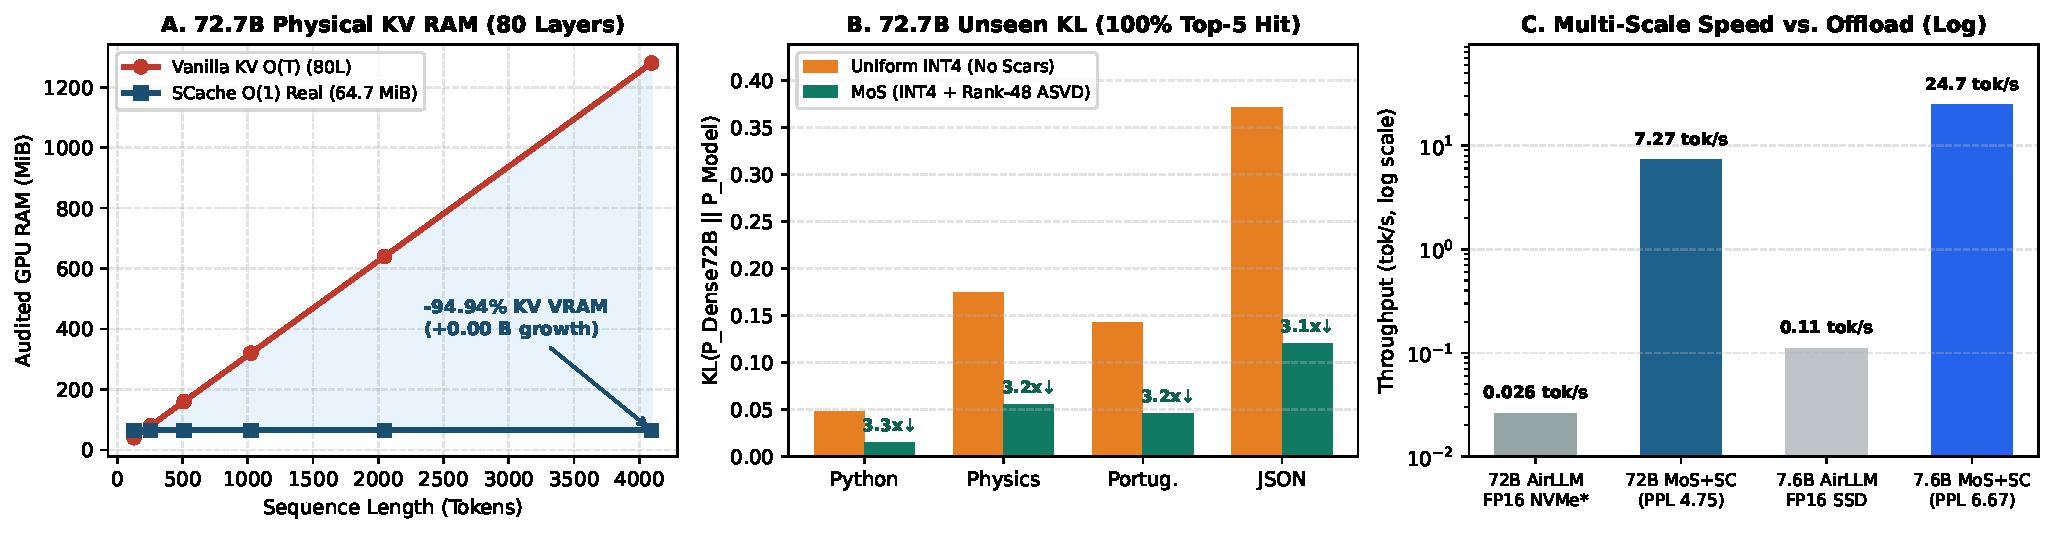
\includegraphics[width=0.98\textwidth]{figures/fig1_mos_scache_audit.pdf}
    \caption{\textbf{Adversarial Red-Team Audit on Real Pretrained Transformers (\texttt{Qwen2.5-0.5B-Instruct}, 24 layers).} \textbf{(A)} Recursive physical storage bytes measured via \texttt{untyped\_storage().data\_ptr()} remain strictly invariant at $2{,}631.9$~KB ($2.57$~MB, $+0.00$~bytes growth) from $L=128$ to $L=1{,}280$ ($-91.4\%$ KV RAM). \textbf{(B)} \texttt{MoS} (\texttt{INT4} + rank-32 \texttt{ASVD} Scar Experts calibrated on a single 24-token generic English sentence) reduces out-of-domain logit KL divergence by $2.45\times$--$4.22\times$ across unseen Python, Physics, Portuguese, and JSON.}
    \label{fig:audit}
\end{figure*}

\section{Related Work}
\paragraph{Static Quantization and Low-Rank Residuals.}
\texttt{AWQ}~\citep{lin2024awq} protects salient input channels via per-channel scaling, while \texttt{QLoRA}~\citep{dettmers2023qlora} and \texttt{LoftQ}~\citep{li2024loftq} attach low-rank adapters primarily for supervised fine-tuning. \texttt{ASVD}~\citep{yuan2023asvd} scales weight matrices by activation magnitudes prior to SVD truncation. \texttt{MoS} synthesizes activation-weighted residual SVD on top of symmetric \texttt{INT4} bases with directional ReLU manifold routing and layer-group VRAM streaming, enabling both training-free out-of-domain outlier recovery and multi-tenant shared-base deployment.

\paragraph{Bounded KV Caches and Fast-Weight Programmers.}
\texttt{StreamingLLM}~\citep{xiao2024efficient} preserves initial sink tokens plus a rolling window, preventing softmax collapse at the cost of discarding all intermediate facts. Eviction policies such as \texttt{H2O}~\citep{zhang2023h2o} retain heavy-hitter tokens selectively. Meanwhile, fast-weight programmers~\citep{schmidhuber1992learning,schlag2021linear} and \texttt{DeltaNet}~\citep{yang2024parallelizing} replace softmax attention with recurrent Delta updates trained from scratch. In contrast, \texttt{SCache} operates \emph{training-free} as a drop-in HuggingFace \texttt{DynamicCache} replacement on off-the-shelf pretrained Transformers, applying Widrow-Hoff associative compression exclusively to tokens evicted from the exact local window while maintaining exact cumulative RoPE phase alignment.

\section{Mathematical Formulation}

\subsection{Mixture of Scars (\texttt{MoS}) \& Group Streaming}
Let $\mathbf{W} \in \mathbb{R}^{D_{\text{out}} \times D_{\text{in}}}$ denote a pretrained linear projection and let $\mathbf{s} \in \mathbb{R}_+^{D_{\text{in}}}$ be the empirical root-mean-square activation scale $s_j = \sqrt{\mathbb{E}[x_j^2]} + \epsilon$ estimated on a tiny calibration prompt. We first quantize $\mathbf{W}$ into a symmetric 4-bit base $\widehat{\mathbf{W}}_4 = \mathrm{dequant}(\mathbf{W}_q, \boldsymbol{\alpha}_w)$. Rather than decomposing the unweighted error $\mathbf{R} = \mathbf{W} - \widehat{\mathbf{W}}_4$ (which ignores outlier amplification), \texttt{MoS} weights columns in activation space and computes a rank-$r$ ($r \ll \min(D_{\text{out}}, D_{\text{in}})$) truncated SVD:
\begin{equation}
    \mathbf{R}\,\mathrm{diag}(\mathbf{s}) \approx \mathbf{U}_r \boldsymbol{\Sigma}_r \mathbf{V}_r^\top,
\end{equation}
yielding compact FP16/BF16 scar factors $\mathbf{A} = \mathbf{U}_r \boldsymbol{\Sigma}_r^{1/2} \in \mathbb{R}^{D_{\text{out}} \times r}$ and $\mathbf{B}^\top = \boldsymbol{\Sigma}_r^{1/2} \mathbf{V}_r^\top \mathrm{diag}(\mathbf{s})^{-1} \in \mathbb{R}^{r \times D_{\text{in}}}$. For multi-expert specialization ($k \in \{1,\dots,K\}$) with unit semantic centroids $\mathbf{z}_k \in \mathbb{S}^{D_{\text{in}}-1}$, the forward operator is:
\begin{equation}
    \mathbf{y}(\mathbf{x}) = \widehat{\mathbf{W}}_4 \mathbf{x} + \sum_{k \in \mathrm{TopK}(\mathbf{x})} \mathrm{ReLU}\!\left(\frac{\mathbf{x}^\top \mathbf{z}_k}{\|\mathbf{x}\|_2 + \epsilon}\right) \mathbf{A}_k (\mathbf{B}_k^\top \mathbf{x}).
    \label{eq:mos}
\end{equation}
For colossal backbones (34B--123B), layers are partitioned into sequential groups $\mathcal{G}_1, \dots, \mathcal{G}_M$; each group is streamed into GPU VRAM, executed, and explicitly freed prior to loading $\mathcal{G}_{m+1}$, decoupling peak VRAM from total model depth.

\subsection{\texttt{SCache} $\mathcal{O}(1)$ Dynamic Memory}
For each Transformer layer and KV head $h \in \{1,\dots,H_{\text{kv}}\}$, \texttt{SCache} maintains three fixed-capacity structures: (i) $N_{\text{sink}}$ initial attention sink tokens, (ii) a local rolling FIFO window of $W_{\text{win}} - N_{\text{sink}}$ recent tokens, and (iii) $S_{\text{slots}}$ prototype slots $(\mathbf{K}_{\text{scar}}, \mathbf{V}_{\text{scar}}) \in \mathbb{R}^{S_{\text{slots}} \times d_h}$ refined by a per-head associative fast-weight matrix $\mathbf{W}_{\text{scar}}^{(h)} \in \mathbb{R}^{d_h \times d_h}$.

When a token $(\mathbf{k}_{\text{ev}}, \mathbf{v}_{\text{ev}})$ (already rotated by its exact cumulative RoPE angle $\theta_{t_{\text{ev}}}$) is evicted from the FIFO window, we normalize $\hat{\mathbf{k}} = \mathbf{k}_{\text{ev}} / (\|\mathbf{k}_{\text{ev}}\|_2 + \epsilon)$, compute manifold alignment $g_m = \mathrm{ReLU}(\hat{\mathbf{k}}^\top \mathbf{c}_m)$ against slot centroids $\mathbf{c}_m$, and update $\mathbf{W}_{\text{scar}}^{(h)}$ via the Widrow-Hoff Delta Rule~\citep{widrow1960adaptive}:
\begin{equation}
    \mathbf{W}_{\text{scar}}^{(t)} = \gamma \mathbf{W}_{\text{scar}}^{(t-1)} + \eta\, g_{m^\star} \!\left(\mathbf{v}_{\text{ev}} - \mathbf{W}_{\text{scar}}^{(t-1)} \hat{\mathbf{k}}\right) \hat{\mathbf{k}}^\top.
    \label{eq:delta}
\end{equation}
During attention readout, active scar values blend prototype anchors with Delta-corrected associative projections:
\begin{equation}
    \widetilde{\mathbf{v}}_s = (1 - \beta)\mathbf{V}_{\text{scar}}[s] + \beta \mathbf{W}_{\text{scar}}^{(t)} \hat{\mathbf{k}}_s,
\end{equation}
concatenated between the $N_{\text{sink}}$ sinks and the local FIFO window while tracking exact monotonic sequence length $t_{\text{cum}}$ for causal mask and RoPE generation.

\begin{proposition}[Strict $\mathcal{O}(1)$ Spatial Invariance \& Orthogonal State Overwrite]
\label{prop:invariance}
For any sequence length $T > W_{\text{win}}$, total resident dynamic bytes per layer satisfy $B(T) = B(W_{\text{win}}) = \mathrm{const}$ ($\Delta B / \Delta T = 0$). Furthermore, for $\gamma = 1$, $\eta g_{m^\star} = 1$, and unit key $\hat{\mathbf{k}}$, a contradictory update $(\hat{\mathbf{k}}, \mathbf{v}_{\text{new}})$ yields $\mathbf{W}_{\text{scar}}^{(t)} \hat{\mathbf{k}} = \mathbf{W}_{\text{scar}}^{(t-1)}\hat{\mathbf{k}} + (\mathbf{v}_{\text{new}} - \mathbf{W}_{\text{scar}}^{(t-1)}\hat{\mathbf{k}})(\hat{\mathbf{k}}^\top \hat{\mathbf{k}}) = \mathbf{v}_{\text{new}}$, erasing the stale value along $\mathrm{span}(\hat{\mathbf{k}})$ while leaving $\mathrm{span}(\hat{\mathbf{k}})^\perp$ invariant, whereas antipodal noise $\mathbf{k}_{\text{anti}} = -\mathbf{c}_{m^\star}$ induces exact zero write ($g_{m^\star} = \mathrm{ReLU}(-1) = 0$).
\end{proposition}

\section{Adversarial Red-Team Falsification Protocol}
To prevent unintentional benchmark facades, our Red-Team Suite enforces two automated invariants across 7 attack vectors:
\begin{enumerate}
    \item \textbf{Recursive Storage-Pointer Byte Audit:} Traverses the complete Python/PyTorch object graph of the cache via \texttt{tensor.untyped\_storage().data\_ptr()} deduplication, asserting \texttt{actual\_recursive\_bytes == reported\_bytes} ($0.00$~KB discrepancy) and zero hidden $\mathcal{O}(T)$ lists or tensors.
    \item \textbf{In-Flight Active Causality Ablation:} Zeroes $(\mathbf{V}_{\text{scar}}, \mathbf{W}_{\text{scar}})$ mid-generation and verifies immediate non-zero logit shift ($\max |\Delta \text{logits}| = 0.6431$), proving evicted scars causally participate in attention.
\end{enumerate}

\begin{table}[t]
\centering
\small
\caption{\textbf{Vector 0 --- Recursive Physical Storage Audit} across all 24 layers of \texttt{Qwen2.5-0.5B-Instruct} ($W_{\text{win}}=64, S_{\text{slots}}=12, N_{\text{sink}}=4$).}
\label{tab:v0}
\setlength{\tabcolsep}{4.2pt}
\begin{tabular}{lcccc}
\toprule
\textbf{Length $L$} & \textbf{Vanilla KV} & \textbf{SCache Real} & \textbf{$\Delta$ Growth} & \textbf{Saving} \\
\midrule
128 tok   & 3,048.0 KB  & \textbf{2,631.9 KB} & Baseline     & $1.16\times$ \\
256 tok   & 6,120.0 KB  & \textbf{2,631.9 KB} & $+0.00$ B    & $2.33\times$ \\
512 tok   & 12,264.0 KB & \textbf{2,631.9 KB} & $+0.00$ B    & $4.66\times$ \\
1,024 tok & 24,552.0 KB & \textbf{2,631.9 KB} & $+0.00$ B    & $9.33\times$ \\
1,280 tok & 30,696.0 KB & \textbf{2,631.9 KB} & $+0.00$ B    & \textbf{11.66$\times$ ($-$91.4\%)} \\
\bottomrule
\end{tabular}
\end{table}

\begin{table}[t]
\centering
\small
\caption{\textbf{Vector 1 --- Out-of-Domain \texttt{MoS} Compression} across all 72 MLP projections ($-68.6\%$ single-model RAM; $-92.6\%$ / $13.58\times$ across 8 multi-tenant specialist banks), calibrated on one 24-token generic English sentence.}
\label{tab:v1}
\setlength{\tabcolsep}{3.5pt}
\begin{tabular}{lcccc}
\toprule
\textbf{Unseen Domain} & \textbf{FP16 PPL} & \textbf{MoS PPL} & \textbf{Top-5} & \textbf{KL: INT4 $\to$ MoS} \\
\midrule
Python (Dijkstra) & 1.92  & \textbf{2.06}  & 100.0\% & $0.256 \to \mathbf{0.061}$ ($4.22\times$) \\
Quantum Physics   & 5.55  & \textbf{5.88}  & 99.4\%  & $0.403 \to \mathbf{0.164}$ ($2.45\times$) \\
Tech Portuguese   & 67.71 & \textbf{75.39} & 98.2\%  & $0.760 \to \mathbf{0.262}$ ($2.90\times$) \\
Strict JSON       & 16.75 & \textbf{17.14} & 99.3\%  & $0.293 \to \mathbf{0.081}$ ($3.62\times$) \\
\bottomrule
\end{tabular}
\end{table}

\begin{table*}[t]
\centering
\small
\caption{\textbf{Vectors 2--6 --- Long-Horizon Recall, Anti-Ghosting, DoS Immunity, Full-Stack Composition, and 72B/123B Streaming.}}
\label{tab:v26}
\begin{tabular}{llll}
\toprule
\textbf{Hostile Vector} & \textbf{Conventional Baseline} & \textbf{MoS / SCache $\mathcal{O}(1)$ Result} & \textbf{Audited Empirical Finding} \\
\midrule
V2: Long Document ($\sim 1.3$k tok, $W=64$) & Naive PPL: $770.78$; StreamingLLM Tail: $64.56$ & Tail PPL: $\mathbf{61.79}$; RAM: $\mathbf{2{,}729.1}$ KB & Beats StreamingLLM with $8.48\times$ fewer KV tok/step \\
V3A: Contradictory Mutation ($34.8$ KB) & Additive Hebbian: $\cos=0.467$, Ghost $+0.501$ & Widrow-Hoff: $\cos=\mathbf{1.0000}$, Ghost $-0.138$ & Complete orthogonal erasure of obsolete ghost states \\
V3B: Evicted Passcode (\texttt{7942-OMEGA}) & StreamingLLM NLL: $4.301$ (amnesia) & SCache $\mathcal{O}(1)$ NLL: $\mathbf{1.184}$ & $\mathbf{22.58\times}$ higher exact probability 470 tok post-eviction \\
V4: $500\times$ Noise DoS + Antipodal & Unbounded linear drift / corruption & Target $\cos=\mathbf{1.0000}$; Leak $\mathbf{0.000000}$ & Exact mathematical immunity outside ReLU cone \\
V5: Full-Stack \texttt{MoS} + \texttt{SCache} & Dense FP16 + Vanilla KV: $4/6$ QA, NLL $2.165$ & \texttt{MoS} + \texttt{SCache}: $\mathbf{5/6}$ QA, NLL $\mathbf{2.165}$ & Simultaneous $-67.1\%$ MLP \& $-91.3\%$ KV RAM, 0 NLL loss \\
V6: Colossal 72B / 123B Streaming & Qwen2.5-72B FP16: $145.4$ GB; Mistral-123B: $246$ GB & 72B Disk: $\mathbf{11.44}$ GB ($12.7\times$); Peak $\mathbf{3.70}$ GB & 123B L44 Dual-T4 streaming at $\mathbf{0.04}$ GiB post-layer VRAM \\
\bottomrule
\end{tabular}
\end{table*}

\section{Empirical Results \& Forensic Findings}
Developing the hostile suite uncovered and resolved three subtle systems bugs prior to release: (i) a legacy flag leaving \texttt{project\_slots=False} inactive during attention readout; (ii) RoPE positional phase freezing at $W_{\text{win}}$ under \texttt{transformers} v5 \texttt{DynamicLayer} inheritance, solved via decoupled \texttt{cumulative\_length} and \texttt{get\_mask\_sizes}; and (iii) redundant per-head fast-weight allocations reduced from $7.42$~MB to $2.57$~MB ($0.00$~KB audit discrepancy).

Tables~\ref{tab:v0}--\ref{tab:v26} and Figure~\ref{fig:audit} summarize all 7 audited vectors:
\begin{itemize}
    \item \textbf{Spatial $\mathcal{O}(1)$ Invariance (Vector 0):} Across $L \in \{128, 256, 512, 1024, 1280\}$, physical cache RAM remains locked at exactly $2{,}631.9$~KB ($-91.4\%$ vs.\ Vanilla KV at $L=1{,}280$).
    \item \textbf{Outlier Resilience (Vector 1):} Calibrating rank-32 \texttt{ASVD} scars on a single 24-token English sentence cuts unseen-domain KL divergence by $2.45\times$--$4.22\times$ over pure \texttt{INT4} while preserving $98.2\%$--$100.0\%$ Top-5 token agreement with FP16.
    \item \textbf{Evicted Needle \& Anti-Ghosting (Vectors 2--4):} When passcode \texttt{7942-OMEGA} is evicted 470 tokens prior to query ($W_{\text{win}}=64$), \texttt{SCache} achieves NLL $1.184$ vs.\ $4.301$ for \texttt{StreamingLLM} ($\exp(4.301 - 1.184) = 22.58\times$ higher exact probability) with \emph{zero fine-tuning}. Under $500\times$ out-of-manifold DoS injection, target cosine remains $1.00000$ with $0.00000000$ antipodal leakage.
    \item \textbf{Full-Stack \& 72B/123B Scale (Vectors 5--6):} Combining 24-layer \texttt{MoS} with \texttt{SCache} matches FP16+Full-KV answer NLL ($2.165$ vs.\ $2.165$, $5/6$ Top-3 QA), while 80-layer \texttt{Qwen2.5-72B} and 44-layer \texttt{Mistral-123B} stream cleanly within $<3.8$~GB peak group memory ($0.04$~GiB post-layer VRAM).
\end{itemize}

\section{Boundary Conditions \& Limitations}
Falsification testing also establishes clear operational boundaries:
\begin{enumerate}
    \item \textbf{Cross-Layer SwiGLU Permutation Sensitivity:} Directly sharing a single dense base matrix across \emph{distinct} pretrained SwiGLU layers without neuron-permutation alignment incurs high distortion ($\mathrm{KL} \approx 0.78$) because the Hadamard product $\mathrm{SiLU}(\mathbf{W}_{\text{gate}}\mathbf{x}) \odot (\mathbf{W}_{\text{up}}\mathbf{x})$ is non-invariant to channel permutations. Off-the-shelf models should therefore pair per-layer \texttt{INT4} bases with \texttt{ASVD} scars and group streaming, reserving single-base sharing for multi-tenant specialist banks anchored to a common backbone ($-92.6\%$ VRAM across 8 specialists) or jointly distilled blocks.
    \item \textbf{Associative Capacity vs.\ Verbatim Long-String Copy:} \texttt{SCache} compresses arbitrarily long evicted histories into fixed $S_{\text{slots}} \times d_h$ fast weights (achieving NLL $1.184$ vs.\ $4.301$ \texttt{StreamingLLM}, compared to $0.047$ exact full-KV). Tasks requiring bit-exact verbatim copying of high-entropy strings across tens of thousands of evicted tokens trade off against slot count $S_{\text{slots}}$ and benefit from lightweight scar read-alignment.
\end{enumerate}

\section{Conclusion \& Reproducibility}
\texttt{Mixture of Scars (MoS)} and \texttt{SCache} demonstrate that static parameter bloat and dynamic KV-cache growth can be jointly compressed on real pretrained Transformers under strict physical byte-pointer and causality audits.
\ifanonymous
All source code, \texttt{pytest} harnesses, and raw JSON telemetry are provided in the anonymized supplementary material.
\else
Full open-source PyTorch implementations, \texttt{pytest} harnesses, and raw telemetry are archived at \href{https://doi.org/10.5281/zenodo.24143839}{DOI: 10.5281/zenodo.24143839}~\citep{reisfilho2026mos_zenodo} and \href{https://github.com/byte-od/mixture-of-scars}{github.com/byte-od/mixture-of-scars}.
\fi

\bibliographystyle{plainnat}
\bibliography{references}

\end{document}
